\chapter{Sezione Sperimentale}
\label{ch:esperimenti}

\section{Dataset utilizzato}
Per quanto riguarda i dataset, è stata condotta una prima fase di ricerca che portato all'utilizzo di LibriSpeech.
LibriSpeech è un dataset audio utilizzato per l’addestramento e la valutazione di modelli di automatic speech recognition (ASR). Il suo punto di forza è la grande quantità di dati disponibili, derivati da audiolibri di pubblico dominio, 
il che lo rende ideale per sviluppare sistemi che comprendano l’inglese parlato in modo naturale. Sono presenti speakers differenti,
bilanciati in termini di sesso e di durata delle tracce audio. Gli audio vengono forniti già normalizzati e puliti da eventuale rumore.
Il dataset è molto adatto per task di Speaker identification e verification in quanto gli audio sono molto chiari e ben distinguibili. \\
I file audio che compongono LibriSpeech provengono dagli audiolibri registrati nel progetto LibriVox, una piattaforma dove volontari 
leggono e registrano opere letterarie di dominio pubblico. Grazie a questa fonte, il dataset offre un ampio spettro di voci, con 
accenti e tonalità diverse, riflettendo meglio la variabilità del parlato umano, permettendo quindi di avere dati il quanto più
possibili generalizzanti.

\section{Dettagli Esperimenti}
In termini implementativi, per quanto riguarda i vari moduli o componenti, le configurazioni sono riportate in tabella Tab.\ref{tab:esperimenticondotti}.
\begin{table}[ht]
    \centering
    \resizebox{\textwidth}{!}{%
        \begin{tabular}{|ll|l|ll|}
        \hline
        \multicolumn{2}{|c|}{\textit{\textbf{Feature Extraction}}} & \multicolumn{1}{c|}{\textit{\textbf{Speaker Identification}}} & \multicolumn{2}{c|}{\textit{\textbf{Speaker Verification}}} \\ \hline
        \multicolumn{1}{|l|}{\textbf{Features used}} & \textbf{Frame Analysis} & \textbf{Model Used} & \multicolumn{1}{l|}{\textbf{Embedding}} & \textbf{Backend} \\ \hline
        \multicolumn{1}{|l|}{25 MFCCs} & \begin{tabular}[c]{@{}l@{}}25ms frame length\\ 10ms frame hop\end{tabular} & DNN & \multicolumn{1}{l|}{Bottle-neck layer} & GMM-UBM \\ \hline
        \multicolumn{1}{|l|}{25 MFCCs} & \begin{tabular}[c]{@{}l@{}}25ms frame length\\ 10ms frame hop\end{tabular} & DNN & \multicolumn{1}{l|}{Last Hidden layer} & GMM-UBM \\ \hline
        \multicolumn{1}{|l|}{25 MFCCs} & \begin{tabular}[c]{@{}l@{}}25ms frame length\\ 10ms frame hop\end{tabular} & RNN & \multicolumn{1}{l|}{Mean Hidden Layers} & GMM-UBM \\ \hline
        \multicolumn{1}{|l|}{25 MFCCs} & \begin{tabular}[c]{@{}l@{}}25ms frame length\\ 10ms frame hop\end{tabular} & CNN+LSTM & \multicolumn{1}{l|}{Mean Hidden Layers} & GMM-UBM \\ \hline
        \multicolumn{1}{|l|}{20 MFCCs} & \begin{tabular}[c]{@{}l@{}}25ms frame length\\ 10ms frame hop\end{tabular} & I-DNN & \multicolumn{1}{l|}{Segment Embedding} & GMM-UBM \\ \hline
        \multicolumn{1}{|l|}{\begin{tabular}[c]{@{}l@{}}24 MFCCs, \\ 24 Delta-MFCCs\\ VAD 30\% energy\end{tabular}} & \begin{tabular}[c]{@{}l@{}}25ms frame length\\ 10ms frame hop\end{tabular} & TDNN & \multicolumn{1}{l|}{X-embedding} & GMM-UBM \\ \hline
        \end{tabular}%
    }
\caption{Riassunto degli esperimenti condotti}
\label{tab:esperimenticondotti}
\end{table}
In particolare si è voluto dare maggior enfasi alla sperimentazione di diversi modelli,
diversi embedding e sopratutto features differenti. Ogni modello viene addestrato su un training e testing set comune, composto dagli audio
degli speaker autorizzati della top 10 di uomini e donne. Come si evince dalla tabella, per quanto riguarda le speech features da dare
in input ai modelli comunque applichiamo analisi short-time. L'analisi short-time deriva dal fatto che vogliamo
estrarre le caratteristiche di uno speaker a livello di frame (che possiamo pensare ad un singolo fonema), cercando di estrarre le features spaziali
e temporali caratteristiche. Proprio per questa possibilità, applichiamo diversi modelli che cercano ognuno di catturare questi aspetti. 
In particolare,per quanto riguarda la I-DNN, ispirata alla rete utilizzata per il calcolo degli I-Embeddings, validi sostituti degli I-Vectors (obsoleti e superati),
descritta in \cite{snyder2017deep}, andiamo ad estrarre embedding a livello di segmento, oltre che di singolo frames. Invece, gli X-Embedding si basano più
sulla rete descritta in \cite{snyder2018x}, ovvero una Temporal Delay Neural Network. 

\section{Risultati sperimentali}
Di seguito verranno riportate sia i risultati della Speaker Identification che Speaker Verification (in termini di EER).
Per quanto riguarda i risultati della prima, si riporta nel complessivo le prestazioni del sistema in termini di macro F1,Accuracy, e Precision
mentre i risultati sulla precisione del singolo speaker sono salvati nei rispettivi notebook python. Discorso analogo per quanto rigaurda il valore di EER.
\begin{table}[ht]
\resizebox{\textwidth}{!}{%
\begin{tabular}{|ll|l|lll|}
\hline
\multicolumn{2}{|c|}{\textit{\textbf{Feature Extraction}}} & \multicolumn{1}{c|}{\textit{\textbf{Speaker Identification}}} & \multicolumn{3}{l|}{\textit{\textbf{Metriche}}} \\ \hline
\multicolumn{1}{|l|}{\textbf{Features used}} & \textbf{Frame Analysis} & \textbf{Model Used} & \multicolumn{1}{l|}{\textbf{Acc}} & \multicolumn{1}{l|}{\textbf{F1}} & \textbf{Precision} \\ \hline
\multicolumn{1}{|l|}{25 MFCCs} & \begin{tabular}[c]{@{}l@{}}25ms frame length\\ 10ms frame hop\end{tabular} & DNN & \multicolumn{1}{l|}{1.0} & \multicolumn{1}{l|}{1.0} & 1.0 \\ \hline
\multicolumn{1}{|l|}{25 MFCCs} & \begin{tabular}[c]{@{}l@{}}25ms frame length\\ 10ms frame hop\end{tabular} & DNN & \multicolumn{1}{l|}{1.0} & \multicolumn{1}{l|}{1.0} & 1.0 \\ \hline
\multicolumn{1}{|l|}{25 MFCCs} & \begin{tabular}[c]{@{}l@{}}25ms frame length\\ 10ms frame hop\end{tabular} & RNN & \multicolumn{1}{l|}{0.97} & \multicolumn{1}{l|}{0.96} & 0.97 \\ \hline
\multicolumn{1}{|l|}{25 MFCCs} & \begin{tabular}[c]{@{}l@{}}25ms frame length\\ 10ms frame hop\end{tabular} & CNN+LSTM & \multicolumn{1}{l|}{0.99} & \multicolumn{1}{l|}{0.99} & 0.99 \\ \hline
\multicolumn{1}{|l|}{20 MFCCs} & \begin{tabular}[c]{@{}l@{}}25ms frame length\\ 10ms frame hop\end{tabular} & I-DNN & \multicolumn{1}{l|}{0.98} & \multicolumn{1}{l|}{0.98} & 0.98 \\ \hline
\multicolumn{1}{|l|}{\begin{tabular}[c]{@{}l@{}}24 MFCCs, \\ 24 Delta-MFCCs\\ VAD 30\% energy\end{tabular}} & \begin{tabular}[c]{@{}l@{}}25ms frame length\\ 10ms frame hop\end{tabular} & TDNN & \multicolumn{1}{l|}{0.94} & \multicolumn{1}{l|}{0.94} & 0.95 \\ \hline
\end{tabular}%
}
\caption{Speaker Identification}
\label{tab:speakeridresult}
\end{table}

\begin{table}[ht]
\resizebox{\textwidth}{!}{%
\begin{tabular}{|ll|l|ll|l|}
\hline
\multicolumn{2}{|c|}{\textit{\textbf{Feature Extraction}}} & \multicolumn{1}{c|}{\textit{\textbf{Speaker Identification}}} & \multicolumn{2}{l|}{\textit{\textbf{Speaker Verification}}} & \multicolumn{1}{c|}{\textit{\textbf{Metrics}}} \\ \hline
\multicolumn{1}{|l|}{\textbf{Features used}} & \textbf{Frame Analysis} & \textbf{Model Used} & \multicolumn{1}{l|}{\textbf{Embedding}} & \textbf{Backend} & \textbf{EER} \\ \hline
\multicolumn{1}{|l|}{25 MFCCs} & \begin{tabular}[c]{@{}l@{}}25ms frame length\\ 10ms frame hop\end{tabular} & DNN & \multicolumn{1}{l|}{Bottle-neck layer} & GMM-UBM & 0.03 \\ \hline
\multicolumn{1}{|l|}{25 MFCCs} & \begin{tabular}[c]{@{}l@{}}25ms frame length\\ 10ms frame hop\end{tabular} & DNN & \multicolumn{1}{l|}{Last Hidden layer} & GMM-UBM & 0.13 \\ \hline
\multicolumn{1}{|l|}{25 MFCCs} & \begin{tabular}[c]{@{}l@{}}25ms frame length\\ 10ms frame hop\end{tabular} & RNN & \multicolumn{1}{l|}{Mean Hidden Layers} & GMM-UBM & 0.12 \\ \hline
\multicolumn{1}{|l|}{25 MFCCs} & \begin{tabular}[c]{@{}l@{}}25ms frame length\\ 10ms frame hop\end{tabular} & CNN+LSTM & \multicolumn{1}{l|}{Mean Hidden Layers} & GMM-UBM & 0.15 \\ \hline
\multicolumn{1}{|l|}{20 MFCCs} & \begin{tabular}[c]{@{}l@{}}25ms frame length\\ 10ms frame hop\end{tabular} & I-DNN & \multicolumn{1}{l|}{I-embedding} & GMM-UBM & 0.16 \\ \hline
\multicolumn{1}{|l|}{\begin{tabular}[c]{@{}l@{}}24 MFCCs, \\ 24 Delta-MFCCs\\ VAD 30\% energy\end{tabular}} & \begin{tabular}[c]{@{}l@{}}25ms frame length\\ 10ms frame hop\end{tabular} & TDNN & \multicolumn{1}{l|}{X-embedding} & GMM-UBM & 0.48 \\ \hline
\end{tabular}%
}
\caption{Speaker Verification}
\label{tab:speakerverresults}
\end{table}

\begin{figure}[ht]
    \centering
    \begin{minipage}{0.47\textwidth}
        \centering
        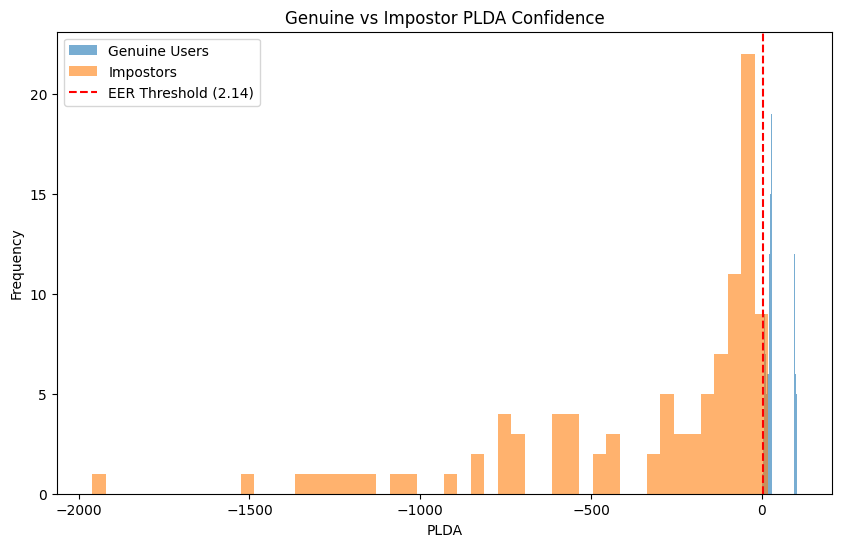
\includegraphics[width=\textwidth]{./ch4/dnn1.png}
        \caption{DNN (1)}
    \end{minipage}
    \begin{minipage}{0.47\textwidth}
        \centering
        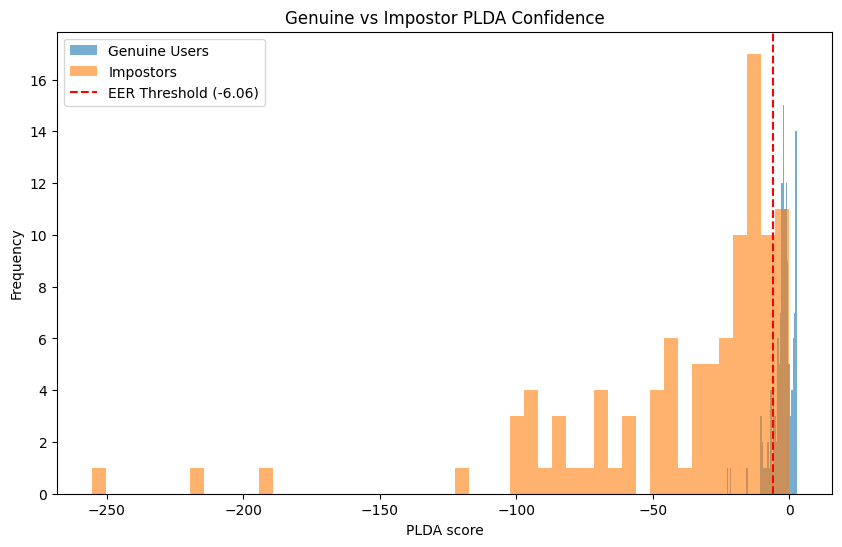
\includegraphics[width=\textwidth]{./ch4/dnn2.png}
        \caption{DNN (2)}
    \end{minipage}

    \begin{minipage}{0.47\textwidth}
        \centering
        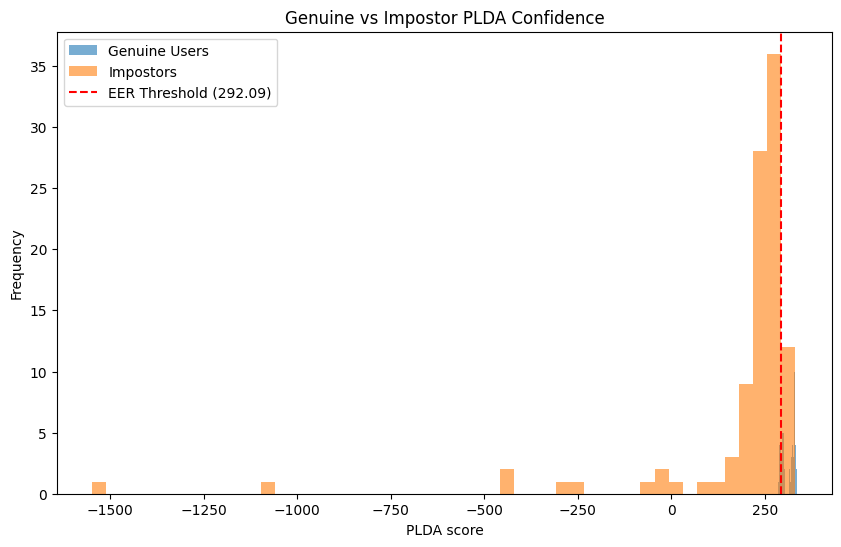
\includegraphics[width=\textwidth]{./ch4/rnn}
        \caption{RNN}
    \end{minipage}
    \begin{minipage}{0.47\textwidth}
        \centering
        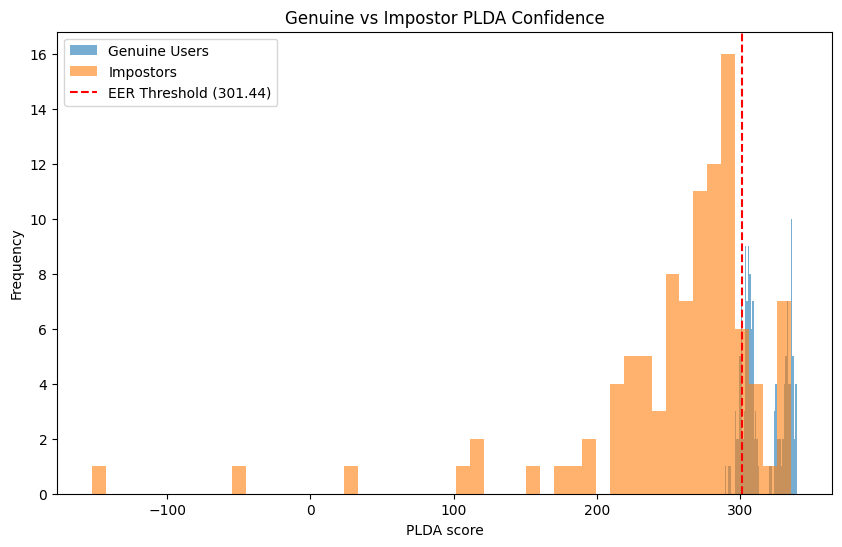
\includegraphics[width=\textwidth]{./ch4/cnnlstm.png}
        \caption{CNN+LSTM}
    \end{minipage}

    \begin{minipage}{0.47\textwidth}
        \centering
        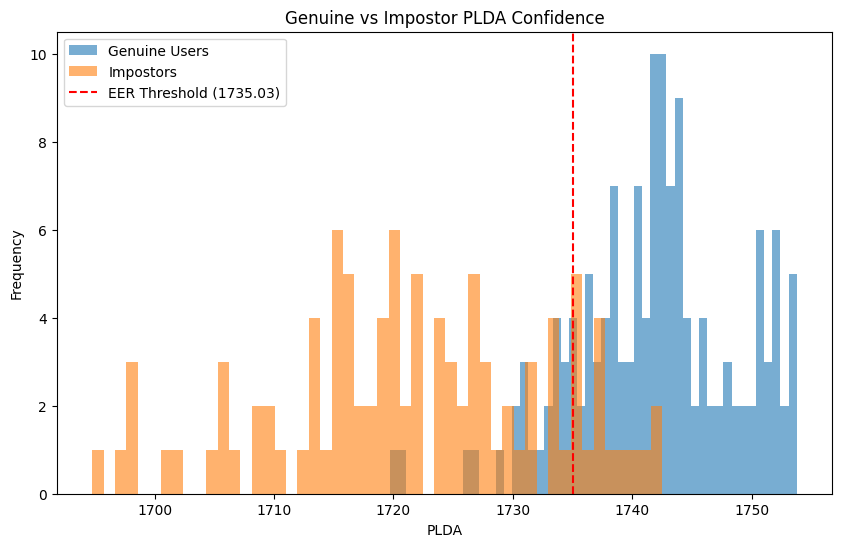
\includegraphics[width=\textwidth]{./ch4/idnn.png}
        \caption{I-DNN}
    \end{minipage}
    \begin{minipage}{0.47\textwidth}
        \centering
        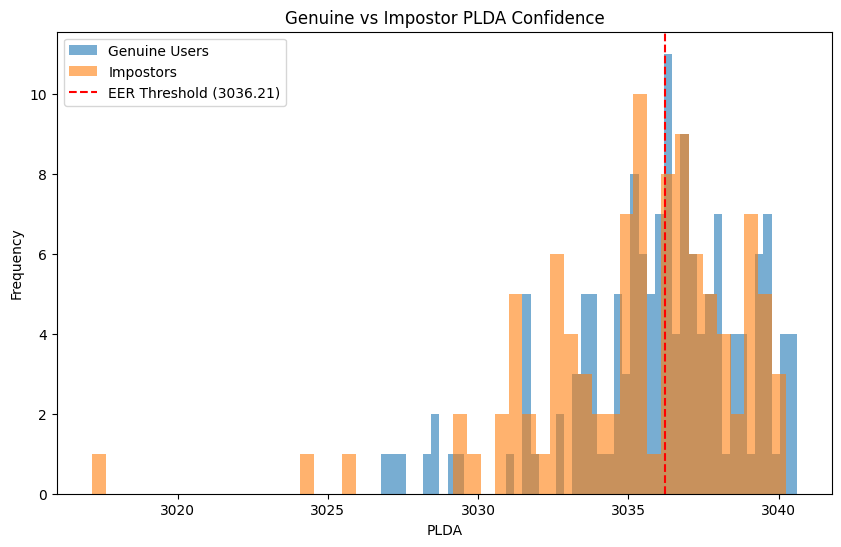
\includegraphics[width=\textwidth]{./ch4/xdnn.png}
        \caption{X-DNN}
    \end{minipage}
\end{figure}


\clearpage

\section{Conclusioni}
Alla luce delle sperimenazioni effettuate, dalla tabella Tab.\ref{tab:speakeridresult} vediamo come effettivamente
tutti i modelli si comportano molto bene nella identificazione degli utenti. Tuttavia va precisato che la natura del dataset non è
di grandi dimensioni, difatti abbiamo a disposizione circa 100 audio per ogni speaker, il che sicuramente è molto limitante come numero. 
Tuttavia, è nella fase di sperimentazione della Speaker Verification (riportate in tabella Tab.\ref{tab:speakerverresults}) dove notiamo che la 
legge del rasoio di Occam non delude mai: difatti la rete che presenta le migliori prestazioni sembra essere la DNN tradizionale cone 
estrazione degli embedding dal Bottleneck.

Difatti entrambe le DNN presentate anche in termini di distribuzione degli scores da parte del backend (vedi Fig.5.1 e Fig.5.2) sia molto precisa
nel trovare embedding abbastanza discriminanti. Discorso diverso invece va fatto per le due ultime reti,
I-DNN e X-DNN, dove vediamo che la distribuzione è abbastanza spalmata e sovrapposta, sintomo che la rete non riesce ancora bene a distinguere. Questo 
lo possiamo notare sopratutto dove la X-DNN riporta il peggior risultato in termini di EER. Questo potrebbe essere dovuto al fatto che la rete
presenta un numero di parametri abbastanza elevato e rischia di overfittare quasi subito, andando difatti a riconoscere bene gli speaker, ma nonr riuscendo
a discriminare quelli "reali" da quelli "estranei". 

Concluendo, possiamo dire che questi sistemi basati su deep learning sul dataset attualmente in uso permettono in maniera precisa di identificare gli speaker,
quindi si prestano molto bene per task in closed-set, ma non possiamo sicuramente dire lo stesso per quanto riguarda il sistema di verifica, che presenta un EER troppo alto,
sintomo che ci sarebbero tanti falsi positivi che riuscirebbero ad entrare nel sistema, venendo identificati erroneamente come utenti legittimi